\clearpage
\appendix
\section{Using the Pi-Radio GUI}
\label{sec:gui}
\raggedbottom% this appendix's pages end naturally (no stretched paragraph gaps)
% generated by tools/crop_gui_screenshots.py -- do not edit
% callout positions on images/gui_shot_<section>.png: fractions, x from the left, y from the bottom
\newcommand{\guiCOOneX}{0.0142}
\newcommand{\guiCOOneY}{0.9083}
\newcommand{\guiCOTwoX}{0.5480}
\newcommand{\guiCOTwoY}{0.7114}
\newcommand{\guiCOThreeX}{0.1368}
\newcommand{\guiCOThreeY}{0.6895}
\newcommand{\guiCOFourX}{0.0231}
\newcommand{\guiCOFourY}{0.4913}
\newcommand{\guiCOFiveX}{0.0231}
\newcommand{\guiCOFiveY}{0.2303}
\newcommand{\guiCOSixX}{0.0486}
\newcommand{\guiCOSixY}{0.6011}
\newcommand{\guiCOSevenX}{0.0368}
\newcommand{\guiCOSevenY}{0.1617}
\newcommand{\guiCOEightX}{0.0368}
\newcommand{\guiCOEightY}{0.3172}

% \guishot{image}{width}{callouts as n/X/Y,...}: a section screenshot with red numbered callouts. A callout whose control
% sits at the left edge goes in the margin just left of the image; otherwise it sits just left of the control.
\newcommand{\guishot}[3]{%
  \begin{tikzpicture}
  \node[anchor=south west, inner sep=0] (img) at (0,0) {\includegraphics[width=#2]{#1}};
  \begin{scope}[x={(img.south east)}, y={(img.north west)}]
  \foreach \n/\X/\Y in {#3}{%
    \pgfmathsetmacro{\cx}{\X < 0.1 ? -0.022 : \X - 0.018}%
    \node[circle, fill=red!80!black, text=white, font=\scriptsize\bfseries, inner sep=1pt, minimum size=10pt]
      at (\cx,\Y) {\n};}
  \end{scope}
  \end{tikzpicture}}

The Pi-Radio GUI is the easiest way to set up the unit. It talks to the unit over the same USB-serial commands listed in
Appendix~\ref{sec:commands}, so anything the GUI can do, a script can do too. This appendix describes GUI version~1.4.1,
for units running firmware~1.4.1. The images are screenshots of the GUI controlling a unit set up for an FR1 of 1\,GHz,
an FR3 of 9\,GHz, and the upper sideband; the red numbers are explained below each image.

\textbf{Starting.} Start the GUI and plug the unit in, in either order. The GUI finds each connected unit by itself and
opens one tab per unit; the line at the top of the tab shows the hardware revision, the unit's serial number, its serial
port, and whether it is connected. Only one program can use a unit's serial port at a time: before using a terminal or a
script, close the GUI or press its \textbf{Disconnect} button, and close the other program before reconnecting the GUI.
Each tab has four sections, top to bottom: the Configuration Helper, Clocking and LO, TX Settings, and RX Settings. Click
a section's title to fold it away.

\par\medskip\noindent\begin{minipage}{\linewidth}\centering
\guishot{images/gui_shot_helper.png}{0.9\linewidth}{1/\guiCOOneX/\guiCOOneY, 2/\guiCOTwoX/\guiCOTwoY}
\captionof{figure}{The Configuration Helper.}\label{fig:gui-helper}
\end{minipage}\par
\begin{enumerate}
\setlength{\itemsep}{2pt}
\item \textbf{FR1, FR3, signal bandwidth, and sideband.} Enter what you want; the GUI works out the LO frequency
  (FR3\,$-$\,FR1 for the upper sideband, FR3\,+\,FR1 for the lower), tunes the synthesizer, and sets the sideband
  switch. If that LO is out of range, it says so, keeps the last valid setting, and suggests trying the other sideband.
\item \textbf{The suggested filter.} The graph shows where the wanted signal (green), its image (red), and the LO
  (black) fall, against the measured response of the filter the GUI suggests for these frequencies (blue). This is the
  ``optimal'' filter used throughout this datasheet. The line under the graph gives an estimate of the image rejection
  it buys, not a measurement (Sections~\ref{sec:sideband-suppression} and~\ref{sec:rx-image-rejection}).
\end{enumerate}

\par\medskip\noindent\begin{minipage}{\linewidth}\centering
\guishot{images/gui_shot_clocking.png}{0.9\linewidth}{3/\guiCOThreeX/\guiCOThreeY, 4/\guiCOFourX/\guiCOFourY,
  5/\guiCOFiveX/\guiCOFiveY}
\captionof{figure}{Clocking and LO.}\label{fig:gui-clocking}
\end{minipage}\par
\begin{enumerate}
\setcounter{enumi}{2}
\setlength{\itemsep}{2pt}
\item \textbf{LO drive.} Leave it on \textbf{Automatic}: the unit then sets the synthesizer's drive from the LO
  frequency, as in every measurement in this datasheet. Unticking it lets you choose a fixed drive level.
\item \textbf{Lock status and temperature.} The synthesizer should read \textbf{LOCKED} when the internal synthesizer (VCO/PLL) is
  engaged. Keep its die temperature
  below 100\,\textdegree C (Section~\ref{sec:summary}).
\item \textbf{Clock and LO source.} Internal or external, for the 10\,MHz reference and for the LO. With an external
  LO, the GUI shows the frequency to feed into the ``LO In'' connector, and the unit switches its internal reference
  off and pauses the automatic LO suppression (item~6).
\end{enumerate}

\par\medskip\noindent\begin{minipage}{\linewidth}\centering
\guishot{images/gui_shot_tx.png}{0.9\linewidth}{6/\guiCOSixX/\guiCOSixY, 7/\guiCOSevenX/\guiCOSevenY}
\captionof{figure}{TX Settings.}\label{fig:gui-tx}
\end{minipage}\par
\begin{enumerate}
\setcounter{enumi}{5}
\setlength{\itemsep}{2pt}
\item \textbf{LO suppression.} Leave \textbf{Automatic LO suppression} on: the unit applies its own factory
  calibration (Section~\ref{sec:lo-suppression}), updated every 2\,seconds as it warms up. The line below says what was
  applied and for which temperature, and the grey line which calibration is stored in the unit.
\item \textbf{TX filter.} With \textbf{Use the Configuration Helper's suggested filter} ticked, the TX filter follows
  the suggestion (item~2). Untick it to choose a filter yourself. The line below shows the filter in use.
\end{enumerate}

\par\medskip\noindent\begin{minipage}{\linewidth}\centering
\guishot{images/gui_shot_rx.png}{0.9\linewidth}{8/\guiCOEightX/\guiCOEightY}
\captionof{figure}{RX Settings.}\label{fig:gui-rx}
\end{minipage}\par
\begin{enumerate}
\setcounter{enumi}{7}
\item \textbf{RX filter.} The same, for the RX side, where the filter is what rejects the image
  (Section~\ref{sec:rx-image-rejection}).
\end{enumerate}

\textbf{To reproduce this datasheet's conditions.} Use the internal clock and LO (item~5), leave the LO drive and the LO
suppression on automatic (items~3 and~6), and leave both filters on the suggested filter (items~7 and~8). The
measurements were made with the unit warm --- the synthesizer at about 70--85\,\textdegree C --- which is
also how it runs after a while in normal use.

\textbf{Messages to look out for.} Two states are shown in colour, because they change what the unit does:
\par\medskip\noindent
\begin{minipage}[t]{0.48\linewidth}
\vspace{0pt}
\centering
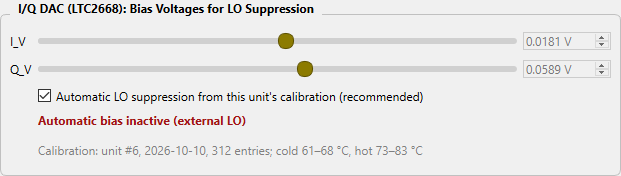
\includegraphics[width=\linewidth]{images/gui_lo_suppr_extlo.png}
\captionof{figure}{External LO selected: the automatic LO suppression is paused (red). The last bias stays applied,
and it is only correct for the frequency it was computed for.}\label{fig:gui-extlo}
\end{minipage}\hfill
\begin{minipage}[t]{0.48\linewidth}
\vspace{0pt}
\centering
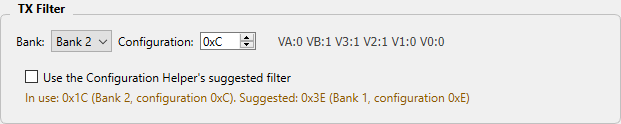
\includegraphics[width=\linewidth]{images/gui_tx_filter_manual.png}
\captionof{figure}{TX filter chosen by hand: the note shows the filter in use and, in amber, the one the Configuration
Helper suggests for the current frequencies.}\label{fig:gui-manual-filter}
\end{minipage}\par
\medskip

\textbf{Nulling the LO yourself.} For the deepest LO suppression in one particular configuration, follow the search in
Section~\ref{sec:lo-suppression}: untick \textbf{Automatic LO suppression} (item~6), then move the I\_V and Q\_V
sliders while watching the LO leakage at the ``TX-side FR3 RF Out'' connector on a spectrum analyzer. Your values stay
applied until you tick the box again, which goes back to the unit's own calibration.

\textbf{Settings the GUI keeps on your computer.} The unit itself remembers every setting it is given (see
Appendix~\ref{sec:commands}). The GUI also remembers, per unit and on the computer it runs on, the FR1, FR3, and signal
bandwidth last entered in the Configuration Helper. If the unit was last set up from another computer, the GUI warns
that these do not match the unit's LO frequency; enter the right values before changing anything else.
\flushbottom
